\documentclass[12pt]{article}
\usepackage{verbatim}
\usepackage[dvips]{epsfig}
\usepackage{color}
\usepackage{url}
\usepackage[colorlinks=true]{hyperref}

\begin{document}

\section*{GENESIS: Documentation}

{\bf Related Documentation:}
% start: userdocs-tag-replace-items related-do-nothing
% end: userdocs-tag-replace-items related-do-nothing

\subsection*{Figure\,12}

\begin{figure}[h]
\centering
   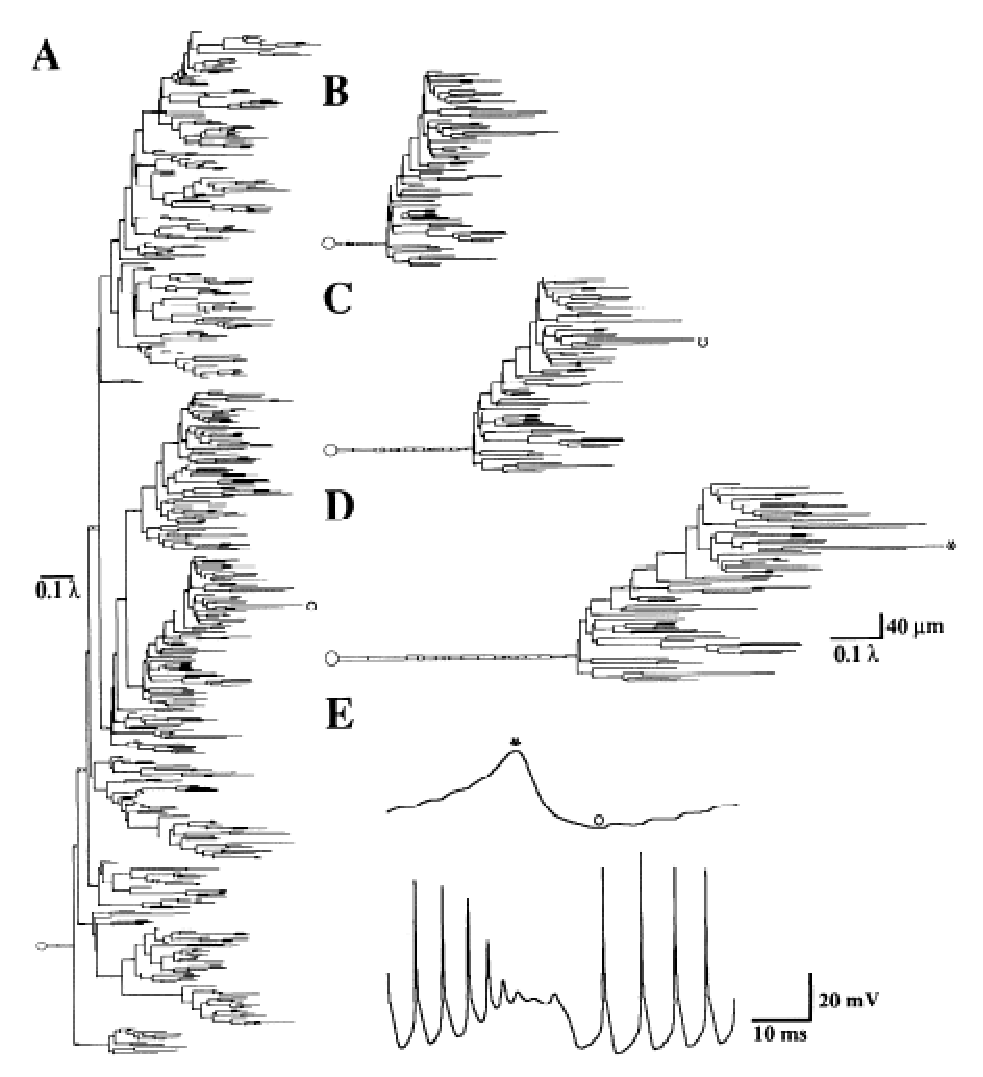
\includegraphics[scale=0.75]{figures/Fig.1.12.eps}
   \caption{Effect of voltage-dependent conductances on the electrotonic length of dendritic segments. {\it A} : Full Sholl diagram in units of electrotonic length of the cell with active conductances in the dendrites, during a pause in between action potentials. {\it B--D}: Enlargement of the Sholl diagram showing the same subset of branchlets (original location indicated by circle in {\it A}) under different conditions of the ionic channels. {\it B}: All passive membrane. {\it C}: Active membrane; the cell is in a quiet state in between action potentials (same as {\it A}). {\it D}: Active membrane at the peak of a dendritic spike. {\it E}: Recording of activity in a spiny dendrite ({\em top trace}, location marked on the Sholl diagrams) and soma ({\em bottom trace}). Dendrogram {\it D} was taken at the time indicated by the asterisk. Dendrogram {\it C} was taken at the time indicated by the circle. Simulation of 2.0\,nA current injection in the soma, model PM9.}
   \label{fig:DS1.12}
\end{figure}

\bibliographystyle{plain}
\bibliography{../tex/bib/g3-refs.bib}

\end{document}
